% Formula sheet for MEC E 371 Heat Transfer
% Two column format

\documentclass[10pt]{article}
\usepackage{amsmath}
\usepackage{amssymb}
\usepackage{multicol}
\usepackage{geometry}
\usepackage{fancyhdr}
\usepackage{siunitx}
\usepackage{enumitem}
\usepackage{multicol}
\usepackage{graphicx}
\usepackage{multirow}
\usepackage{lastpage}
\usepackage[final]{hyperref}
\usepackage{parskip}
\usepackage{subcaption}
\usepackage{float}
\usepackage{pdfpages}

\geometry{letterpaper, portrait, margin=0.5in, footskip=0.25in, top = 0.75in, headsep=0.25in}
\setlength{\columnsep}{0.5in}

\hypersetup{
	colorlinks=true,       % false: boxed links; true: colored links
	linkcolor=blue,        % color of internal links
	citecolor=blue,        % color of links to bibliography
	filecolor=magenta,     % color of file links
	urlcolor=blue         
}

\pagestyle{fancy}
\fancyhf{}
\lhead{MEC E 380 Formula Sheet}
\chead{Last Updated: \today}
\rhead{Alex Diep}
\cfoot{\thepage\ of \pageref{LastPage}}

\begin{document}
%\maketitle
%\thispagestyle{empty}
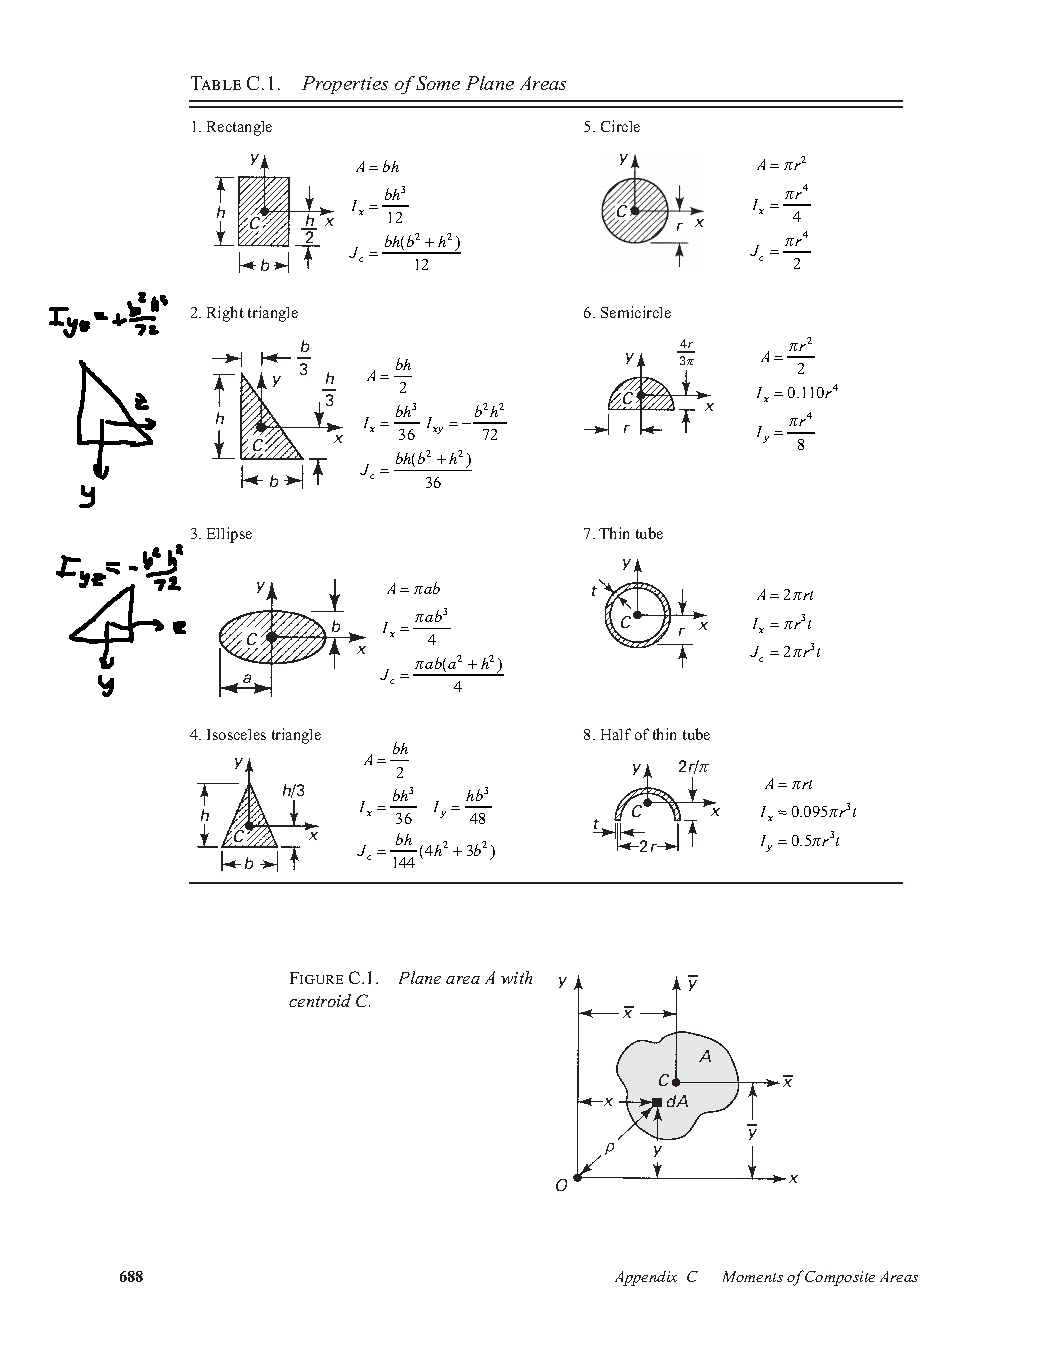
\includepdf[pages=-]{properties_of_some_plane_areas.pdf}
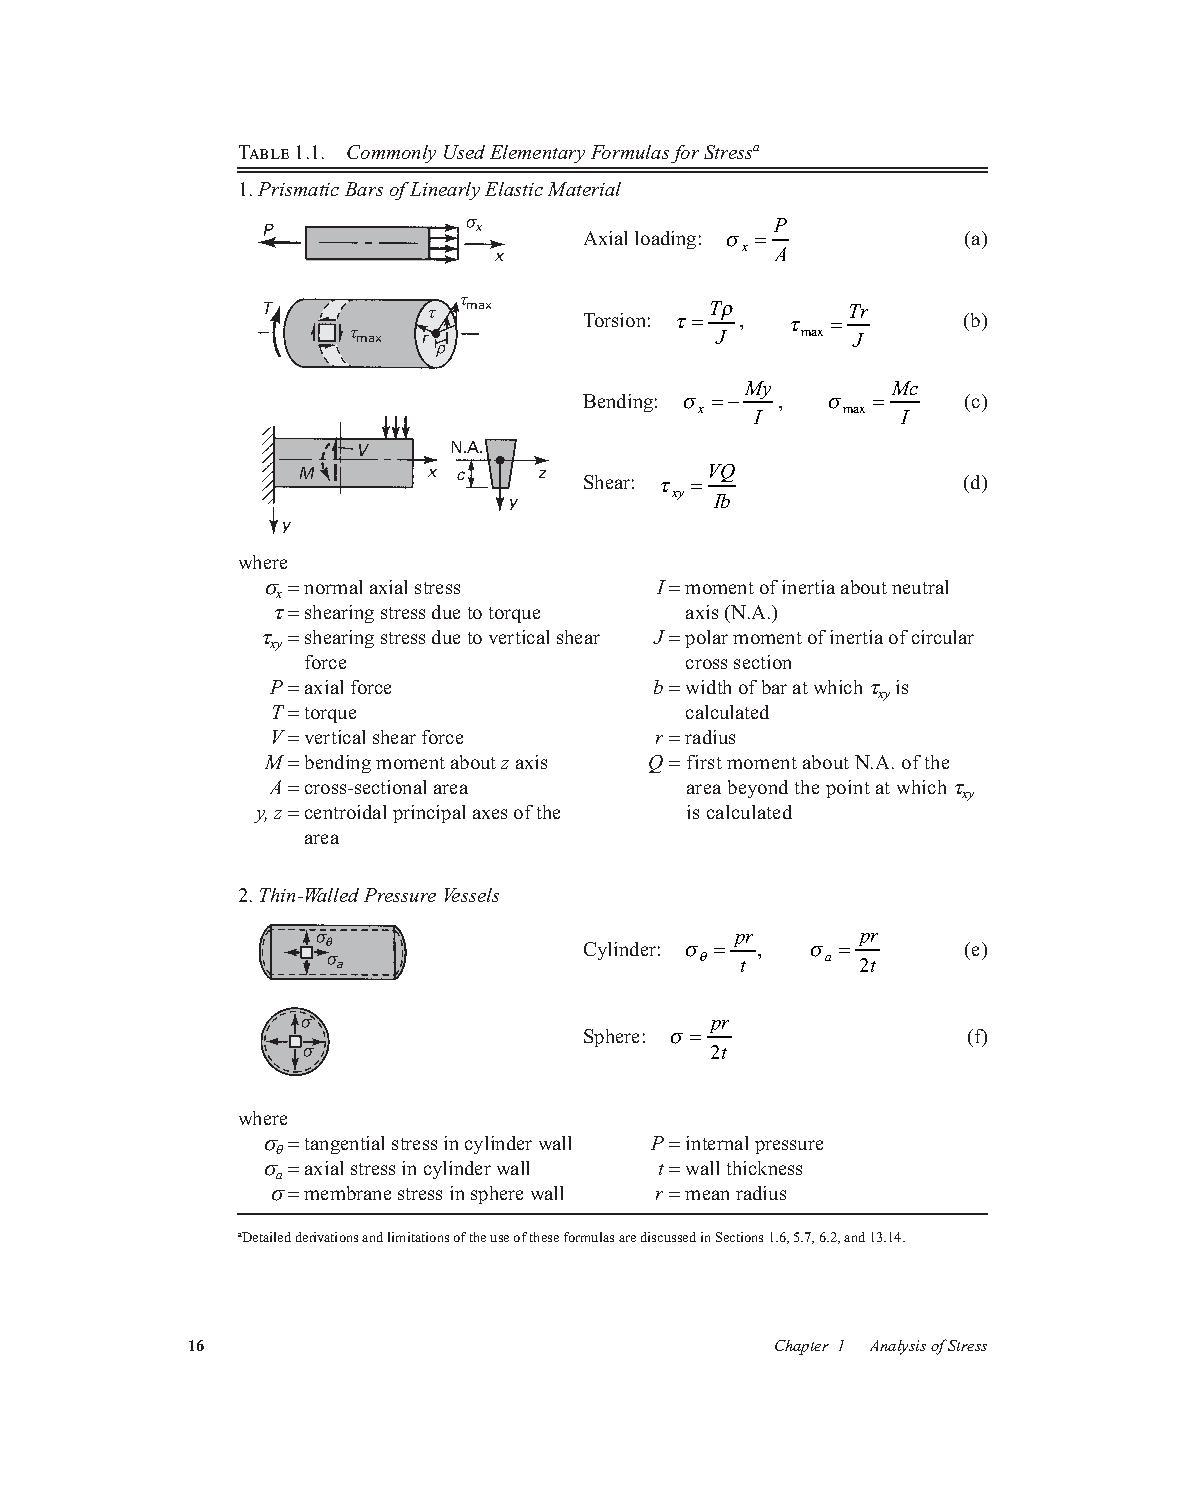
\includepdf[pages=-]{elementary_formulas.pdf}
\begin{multicols*}{2}
\setlength{\belowdisplayskip}{5pt} \setlength{\belowdisplayshortskip}{0pt}
\setlength{\abovedisplayskip}{5pt} \setlength{\abovedisplayshortskip}{0pt}
\section*{5. Bending of Beams}
\subsection*{5.1. General Procedure}
General procedure of asymmetric bending problems
\begin{enumerate}
    \item Identify the location of the centroid of the cross-section, and define it as the origin of the $(y, z)$ coordinate system.
    If the centroid is unknown, set an arbitrary origin and use parallel axis theorem to find the centroid.
    \item Define the orientation of $(y, z)$ axes of the cross-section wisely so that all required moments of 
    inertia $I_y$, $I_z$, and $I_{yz}$ can be obtained (from Table) or calculated easily.
    \item Determine bending moments $M_z$ and $M_y$ at your cross-section. Use elementary beam theory to find the bending moments 
    if given a load.
    \item Use the relations to find the stress $\sigma_x$ and the neutral axis.
\end{enumerate}
\subsection*{5.2. Formulas}
Centroid equations:
\begin{align*}
    \bar{x} &= \frac{\sum \bar{x}_i A_i}{\sum A_i} 
\end{align*}
where $\bar{x}_i$ is the $x$-coordinate of the centroid of the $i$-th area, and $A_i$ is the area of the $i$-th area.

Moment equations:
\begin{gather*}
    M_y = P_z L \\
    M_z = P_y L 
\end{gather*}
where $P_z$ and $P_y$ are positive in the positive $z$ and $y$ directions, respectively.
Parallel axis theorem:
\begin{gather*}
    \bar{z} = \frac{\sum \bar{z}_i A_i}{\sum A_i} \\
    \bar{y} = \frac{\sum \bar{y}_i A_i}{\sum A_i} \\
    I_z = \sum(I_{\bar{z}, i} + A_i d_{y, i}^2) \\
    I_y = \sum(I_{\bar{y}, i} + A_i d_{z, i}^2) \\
    I_{yz} = \sum(I_{\bar{yz}, i} + A_i d_{y, i} d_{z, i}) 
\end{gather*}
where $I_{\bar{z}, i}$, $I_{\bar{y}, i}$, and $I_{\bar{yz}, i}$ are the moments of inertia about the centroidal axes, 
and $d_{y, i}$ and $d_{z, i}$ are the distances from the centroidal axes to the parallel axes. Note:
$I_{yz} = 0$ if there is symmetry about \textbf{either} the $y$ or $z$ direction.

Moment to stress:
\begin{gather*}
    \tau = \frac{VQ}{Ib} \overset{\text{rect}}{=} \frac{3V}{2A_c} \\
    \sigma_{x} = \frac{(M_y I_z + M_z I_{yz})d_{z} - (M_y I_{yz} + M_z I_y)d_{y}}{I_y I_z - I_{yz}^2} \\
    \tan{\phi} = \frac{M_y I_z + M_z I_{yz}}{M_z I_y + M_y I_{yz}} 
\end{gather*}
stress is maximum at the furthest point from the neutral axis on the cross-section. For $\sigma_x$, 
$d_y$ and $d_z$ are the signed displacements ($\pm$) from the centroid to the point of interest in the $y$ and $z$ directions.

Method of integration
\begin{align*}
    EI \frac{d^4 v}{dx^4} &= p \\
    EI \frac{d^3 v}{dx^3} &= -V \\ 
    EI \frac{d^2 v}{dx^2} &= M \\
    EI \frac{dv}{dx} &= \int M 
\end{align*}
also slope $\theta = dv/dx$ and deflection is $v$.

Singularity functions
\begin{figure}[H]
    \centering
    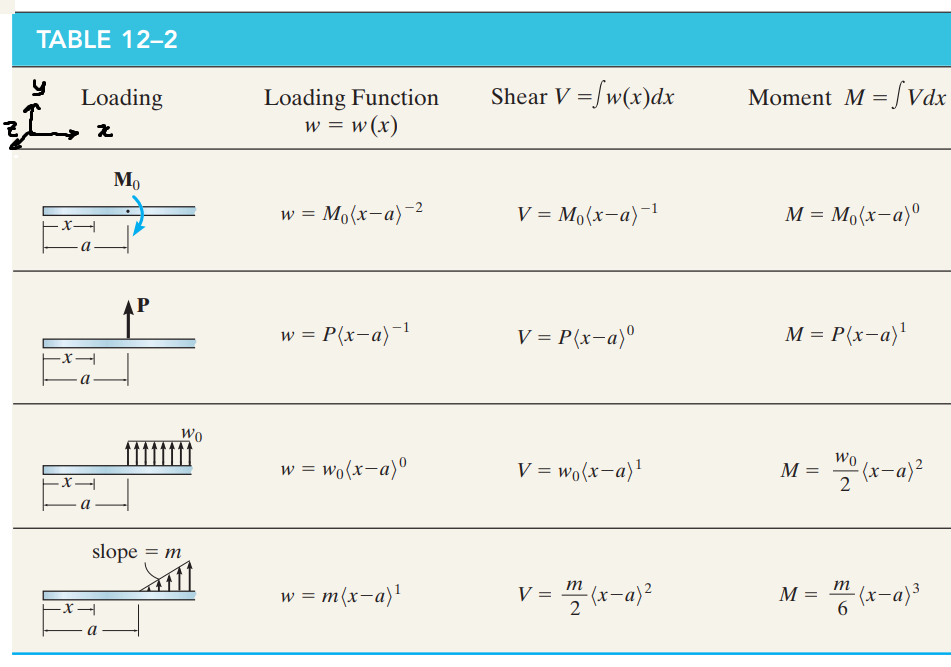
\includegraphics[width=1\linewidth]{Figures/sec5 singularity.png}
    \caption{Singularity functions}
    \label{fig:sec5 singularity functions}
\end{figure}
where 
\begin{figure}[H]
    \centering
    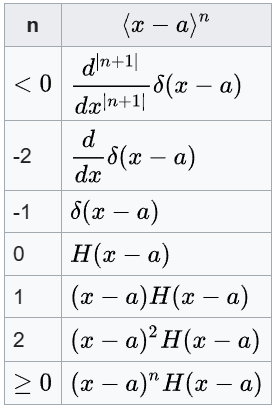
\includegraphics[width=0.5\linewidth]{Figures/sec10 singularity.png}
\end{figure}

\end{multicols*}
\end{document}
